\documentclass{article}

\usepackage{algorithmic}
\usepackage{amstext}
\usepackage{tikz}
\usetikzlibrary{arrows,decorations.pathmorphing,fit,positioning,calc}

\newcommand{\dir}{\text{Dirichlet}}
\newcommand{\mult}{\text{Multinomial}}

\begin{document}

\section{Plate Diagram}

\begin{figure}[htp]
  \centering
  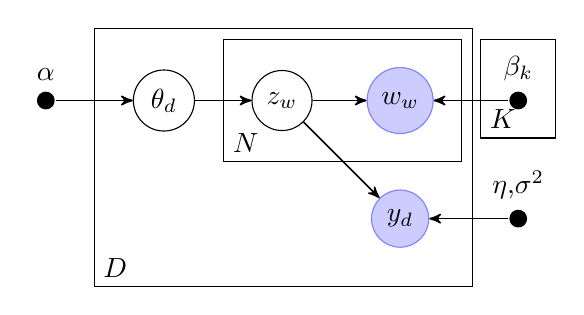
\begin{tikzpicture}
    [
      observed/.style={minimum size=15pt,circle,draw=blue!50,fill=blue!20},
      unobserved/.style={minimum size=15pt,circle,draw},
      hyper/.style={minimum size=1pt,circle,fill=black},
      post/.style={->,>=stealth',semithick},
    ]

    \node (w-w) [observed] at (0,0) {$w_w$};
    \node (y-d) [observed] at (0,-1.5) {$y_d$};
    \node (y-prior) [label=above:$\eta\text{,}\sigma^2$] at (1.5,-1.5) {};
    \filldraw [black] (1.5,-1.5) circle (3pt);
    \node (z-w) [unobserved] at (-1.5,0) {$z_w$};
    \node (z-prior) [unobserved] at (-3,0) {$\theta_d$};
    \node (z-hyper) [label=above:$\alpha$] at (-4.5,0) {};
    \filldraw [black] (-4.5,0) circle (3pt);
    \node (beta) [label=above:$\beta_k$] at (1.5,0) {};
    \filldraw [black] (1.5,0) circle (3pt);
    \node (beta-label) at (1.5,0.3) {};
    
    \path
    (z-w) edge [post] (w-w)
    (z-w) edge [post] (y-d)
    
    (z-hyper) edge [post] (z-prior)
    (y-prior) edge [post] (y-d)
    (z-prior) edge [post] (z-w)

    (beta) edge [post] (w-w)
    ;

    \node [draw,fit=(beta) (beta-label), inner sep=10pt] (plate-topics) {};
    \node [above right] at (plate-topics.south west) {$K$};
    \node [draw,fit=(w-w) (z-prior) (y-d), inner sep=14pt] (plate-context) {};
    \node [above right] at (plate-context.south west) {$D$};
    \node [draw,fit=(w-w) (z-w), inner sep=10pt] (plate-token) {};
    \node [above right] at (plate-token.south west) {$N$};

  \end{tikzpicture}
  \caption{Plate Diagram of LDA. For more information, see \cite{Blei:2007} }
  \label{fig:graphical-model}
\end{figure}

\section{Equations}
See~\cite{Blei:2007}.
\subsection{Generative Process}
\begin{algorithmic}[1]
  \FOR{document $d_d$ in corpus $D$}
  \STATE Choose $\theta_d \sim \dir(\alpha) $
  \FOR{position $w$ in $d_d$}
    \STATE Choose a topic $z_w \sim \mult(\theta_d)$
    \STATE Choose a word $w_w | z_w,\beta_k \sim \mult(\beta_{z_w})$
  \ENDFOR
  \ENDFOR
\end{algorithmic}

\bibliographystyle{plain}
\bibliography{tm}

\end{document}
